% Options for packages loaded elsewhere
\PassOptionsToPackage{unicode}{hyperref}
\PassOptionsToPackage{hyphens}{url}
%
\documentclass[
]{article}
\usepackage{amsmath,amssymb}
\usepackage{lmodern}
\usepackage{iftex}
\ifPDFTeX
  \usepackage[T1]{fontenc}
  \usepackage[utf8]{inputenc}
  \usepackage{textcomp} % provide euro and other symbols
\else % if luatex or xetex
  \usepackage{unicode-math}
  \defaultfontfeatures{Scale=MatchLowercase}
  \defaultfontfeatures[\rmfamily]{Ligatures=TeX,Scale=1}
\fi
% Use upquote if available, for straight quotes in verbatim environments
\IfFileExists{upquote.sty}{\usepackage{upquote}}{}
\IfFileExists{microtype.sty}{% use microtype if available
  \usepackage[]{microtype}
  \UseMicrotypeSet[protrusion]{basicmath} % disable protrusion for tt fonts
}{}
\makeatletter
\@ifundefined{KOMAClassName}{% if non-KOMA class
  \IfFileExists{parskip.sty}{%
    \usepackage{parskip}
  }{% else
    \setlength{\parindent}{0pt}
    \setlength{\parskip}{6pt plus 2pt minus 1pt}}
}{% if KOMA class
  \KOMAoptions{parskip=half}}
\makeatother
\usepackage{xcolor}
\IfFileExists{xurl.sty}{\usepackage{xurl}}{} % add URL line breaks if available
\IfFileExists{bookmark.sty}{\usepackage{bookmark}}{\usepackage{hyperref}}
\hypersetup{
  pdftitle={R Project Milestone 3},
  pdfauthor={Moyra Rasheed, Courtney Coon, Jarett Maycott},
  hidelinks,
  pdfcreator={LaTeX via pandoc}}
\urlstyle{same} % disable monospaced font for URLs
\usepackage[margin=1in]{geometry}
\usepackage{color}
\usepackage{fancyvrb}
\newcommand{\VerbBar}{|}
\newcommand{\VERB}{\Verb[commandchars=\\\{\}]}
\DefineVerbatimEnvironment{Highlighting}{Verbatim}{commandchars=\\\{\}}
% Add ',fontsize=\small' for more characters per line
\usepackage{framed}
\definecolor{shadecolor}{RGB}{248,248,248}
\newenvironment{Shaded}{\begin{snugshade}}{\end{snugshade}}
\newcommand{\AlertTok}[1]{\textcolor[rgb]{0.94,0.16,0.16}{#1}}
\newcommand{\AnnotationTok}[1]{\textcolor[rgb]{0.56,0.35,0.01}{\textbf{\textit{#1}}}}
\newcommand{\AttributeTok}[1]{\textcolor[rgb]{0.77,0.63,0.00}{#1}}
\newcommand{\BaseNTok}[1]{\textcolor[rgb]{0.00,0.00,0.81}{#1}}
\newcommand{\BuiltInTok}[1]{#1}
\newcommand{\CharTok}[1]{\textcolor[rgb]{0.31,0.60,0.02}{#1}}
\newcommand{\CommentTok}[1]{\textcolor[rgb]{0.56,0.35,0.01}{\textit{#1}}}
\newcommand{\CommentVarTok}[1]{\textcolor[rgb]{0.56,0.35,0.01}{\textbf{\textit{#1}}}}
\newcommand{\ConstantTok}[1]{\textcolor[rgb]{0.00,0.00,0.00}{#1}}
\newcommand{\ControlFlowTok}[1]{\textcolor[rgb]{0.13,0.29,0.53}{\textbf{#1}}}
\newcommand{\DataTypeTok}[1]{\textcolor[rgb]{0.13,0.29,0.53}{#1}}
\newcommand{\DecValTok}[1]{\textcolor[rgb]{0.00,0.00,0.81}{#1}}
\newcommand{\DocumentationTok}[1]{\textcolor[rgb]{0.56,0.35,0.01}{\textbf{\textit{#1}}}}
\newcommand{\ErrorTok}[1]{\textcolor[rgb]{0.64,0.00,0.00}{\textbf{#1}}}
\newcommand{\ExtensionTok}[1]{#1}
\newcommand{\FloatTok}[1]{\textcolor[rgb]{0.00,0.00,0.81}{#1}}
\newcommand{\FunctionTok}[1]{\textcolor[rgb]{0.00,0.00,0.00}{#1}}
\newcommand{\ImportTok}[1]{#1}
\newcommand{\InformationTok}[1]{\textcolor[rgb]{0.56,0.35,0.01}{\textbf{\textit{#1}}}}
\newcommand{\KeywordTok}[1]{\textcolor[rgb]{0.13,0.29,0.53}{\textbf{#1}}}
\newcommand{\NormalTok}[1]{#1}
\newcommand{\OperatorTok}[1]{\textcolor[rgb]{0.81,0.36,0.00}{\textbf{#1}}}
\newcommand{\OtherTok}[1]{\textcolor[rgb]{0.56,0.35,0.01}{#1}}
\newcommand{\PreprocessorTok}[1]{\textcolor[rgb]{0.56,0.35,0.01}{\textit{#1}}}
\newcommand{\RegionMarkerTok}[1]{#1}
\newcommand{\SpecialCharTok}[1]{\textcolor[rgb]{0.00,0.00,0.00}{#1}}
\newcommand{\SpecialStringTok}[1]{\textcolor[rgb]{0.31,0.60,0.02}{#1}}
\newcommand{\StringTok}[1]{\textcolor[rgb]{0.31,0.60,0.02}{#1}}
\newcommand{\VariableTok}[1]{\textcolor[rgb]{0.00,0.00,0.00}{#1}}
\newcommand{\VerbatimStringTok}[1]{\textcolor[rgb]{0.31,0.60,0.02}{#1}}
\newcommand{\WarningTok}[1]{\textcolor[rgb]{0.56,0.35,0.01}{\textbf{\textit{#1}}}}
\usepackage{graphicx}
\makeatletter
\def\maxwidth{\ifdim\Gin@nat@width>\linewidth\linewidth\else\Gin@nat@width\fi}
\def\maxheight{\ifdim\Gin@nat@height>\textheight\textheight\else\Gin@nat@height\fi}
\makeatother
% Scale images if necessary, so that they will not overflow the page
% margins by default, and it is still possible to overwrite the defaults
% using explicit options in \includegraphics[width, height, ...]{}
\setkeys{Gin}{width=\maxwidth,height=\maxheight,keepaspectratio}
% Set default figure placement to htbp
\makeatletter
\def\fps@figure{htbp}
\makeatother
\setlength{\emergencystretch}{3em} % prevent overfull lines
\providecommand{\tightlist}{%
  \setlength{\itemsep}{0pt}\setlength{\parskip}{0pt}}
\setcounter{secnumdepth}{-\maxdimen} % remove section numbering
\usepackage{booktabs}
\usepackage{longtable}
\usepackage{array}
\usepackage{multirow}
\usepackage{wrapfig}
\usepackage{float}
\usepackage{colortbl}
\usepackage{pdflscape}
\usepackage{tabu}
\usepackage{threeparttable}
\usepackage{threeparttablex}
\usepackage[normalem]{ulem}
\usepackage{makecell}
\usepackage{xcolor}
\ifLuaTeX
  \usepackage{selnolig}  % disable illegal ligatures
\fi

\title{R Project Milestone 3}
\author{Moyra Rasheed, Courtney Coon, Jarett Maycott}
\date{2022-11-26}

\begin{document}
\maketitle

\hypertarget{visualization-1}
\DocumentationTok{\#\# median age median = 37.05}
\DocumentationTok{\#\# population density 1st quantile (low cutoff) = 25.887}
\DocumentationTok{\#\# population density 3rd quantile (high cutoff) = 333.485}
\FunctionTok{ggplot}\NormalTok{(}\AttributeTok{data =}\NormalTok{ merged\_data, }\FunctionTok{aes}\NormalTok{(}\AttributeTok{x =}\NormalTok{ renter\_ratio, }\AttributeTok{y =}\NormalTok{ med\_age)) }\SpecialCharTok{+} 
\FunctionTok{geom\_point}\NormalTok{(}\AttributeTok{data =}\NormalTok{ merged\_data, }\FunctionTok{aes}\NormalTok{(}\AttributeTok{x =}\NormalTok{ renter\_ratio, }\AttributeTok{y =}\NormalTok{ med\_age, }
                                   \AttributeTok{color =}\NormalTok{ pop12\_sqmi\_CAT)) }\SpecialCharTok{+}
\FunctionTok{geom\_text\_repel}\NormalTok{(}\FunctionTok{aes}\NormalTok{(}\AttributeTok{label=}\FunctionTok{ifelse}\NormalTok{((med\_age }\SpecialCharTok{\textgreater{}} \DecValTok{37} \SpecialCharTok{\&}\NormalTok{ renter\_ratio }\SpecialCharTok{\textgreater{}} \FloatTok{0.39} 
    \SpecialCharTok{\&}\NormalTok{ (pop12\_sqmi\_CAT}\SpecialCharTok{==}\StringTok{"High priority"}\SpecialCharTok{|}\NormalTok{ pop12\_sqmi\_CAT}\SpecialCharTok{==}\StringTok{"Medium priority"}\NormalTok{)), }
\NormalTok{    county, }\StringTok{""}\NormalTok{)))}\SpecialCharTok{+}
  \FunctionTok{labs}\NormalTok{(}\AttributeTok{title =} \StringTok{"Priority counties identified based on demographic data only:"}\NormalTok{,}
\AttributeTok{subtitle =} \StringTok{"counties with high median age (\textgreater{}37yo), high ratio of renters (\textgreater{}39\%), }
\StringTok{and low or medium population density (\textless{}333 people/sqmi)"}\NormalTok{, }
       \AttributeTok{x =} \StringTok{"Ratio of renters to homeowners"}\NormalTok{, }
       \AttributeTok{y =} \StringTok{"Median age of county residents"}\NormalTok{, }
       \AttributeTok{color =} 
         \FunctionTok{bquote}\NormalTok{(}\FunctionTok{atop}\NormalTok{(Population}\SpecialCharTok{\textasciitilde{}}\NormalTok{per}\SpecialCharTok{\textasciitilde{}}\NormalTok{mile}\SpecialCharTok{\^{}}\NormalTok{\{}\StringTok{"2"}\NormalTok{\}, }\StringTok{"rural as high priority"}\NormalTok{)))}\SpecialCharTok{+}
  \FunctionTok{theme}\NormalTok{(}\AttributeTok{plot.title=}\FunctionTok{element\_text}\NormalTok{(}\AttributeTok{hjust=}\FloatTok{0.5}\NormalTok{),}
        \AttributeTok{plot.subtitle=}\FunctionTok{element\_text}\NormalTok{(}\AttributeTok{hjust=}\FloatTok{0.5}\NormalTok{))}
\end{Highlighting}
\end{Shaded}

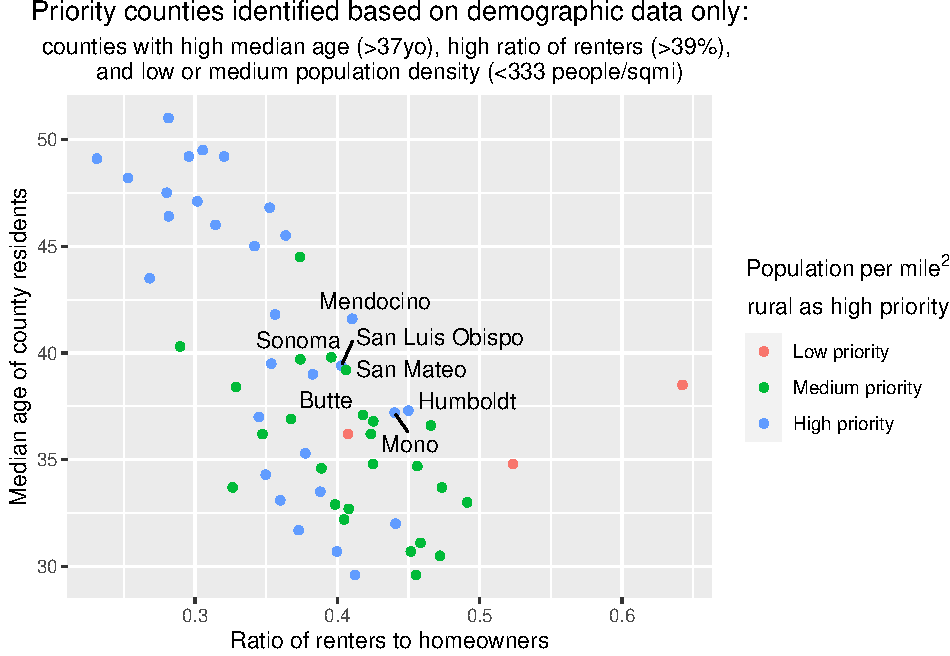
\includegraphics{Milestone-4-R-Project_files/figure-latex/unnamed-chunk-6-1.pdf}

\newpage

\hypertarget{visualization-2}{%
\section{Visualization 2:}\label{visualization-2}}

Plot 2: Here we integrated demographic data from Plot 1 with additional
data: the total dollars invested in prior projects (with higher priority
for less money previously invested) and number of chronic disease
mortality events between 2015-2020, relativized by total population
(with higher priority being higher relative levels of chronic disease
mortality). We used demographic data from Plot 1 to create a new ranked
variable which we used to color code data in Plot 2. Counties
highlighted in Plot 1 were ranked more highly in Plot 2. Thus this Plot
includes all 5 variables of interest to identify the counties that
require greater funding. Note that money invested in previous projects
has been logged to make the plot easier to read.

\begin{Shaded}
\begin{Highlighting}[]
\CommentTok{\# make data set with continuous data and ranking factor for the demographic }
\CommentTok{\# data in the first figure}
\NormalTok{second\_fig\_data\_temp}\OtherTok{\textless{}{-}}\NormalTok{merged\_data}\SpecialCharTok{\%\textgreater{}\%}
  \FunctionTok{select}\NormalTok{(}\FunctionTok{c}\NormalTok{(}\StringTok{"county"}\NormalTok{, }\StringTok{"pop12\_sqmi\_CAT"}\NormalTok{, }\StringTok{"med\_age\_CAT"}\NormalTok{, }\StringTok{"renter\_ratio\_CAT"}\NormalTok{))}\SpecialCharTok{\%\textgreater{}\%}
 \FunctionTok{rowwise}\NormalTok{() }\SpecialCharTok{\%\textgreater{}\%}
 \FunctionTok{mutate}\NormalTok{(}\AttributeTok{number\_highs=} \FunctionTok{sum}\NormalTok{(}\FunctionTok{c\_across}\NormalTok{(}\DecValTok{2}\SpecialCharTok{:}\DecValTok{4}\NormalTok{) }\SpecialCharTok{==} \StringTok{"High priority"}\NormalTok{, }\AttributeTok{na.rm =} \ConstantTok{TRUE}\NormalTok{),}
        \AttributeTok{number\_mediums=} \FunctionTok{sum}\NormalTok{(}\FunctionTok{c\_across}\NormalTok{(}\DecValTok{2}\SpecialCharTok{:}\DecValTok{4}\NormalTok{) }\SpecialCharTok{==} \StringTok{"Medium priority"}\NormalTok{, }\AttributeTok{na.rm =} \ConstantTok{TRUE}\NormalTok{),}
        \AttributeTok{demo\_rank=}\NormalTok{(number\_highs}\SpecialCharTok{*}\DecValTok{2}\NormalTok{)}\SpecialCharTok{+}\NormalTok{number\_mediums}
\NormalTok{        )}\SpecialCharTok{\%\textgreater{}\%}
  \FunctionTok{ungroup}\NormalTok{()}\SpecialCharTok{\%\textgreater{}\%}
  \FunctionTok{select}\NormalTok{(}\FunctionTok{c}\NormalTok{(}\StringTok{"county"}\NormalTok{, }\StringTok{"demo\_rank"}\NormalTok{))}
  
\NormalTok{second\_fig\_data\_final}\OtherTok{\textless{}{-}}\FunctionTok{full\_join}\NormalTok{(second\_fig\_data\_temp, merged\_data, }\AttributeTok{by=}\StringTok{"county"}\NormalTok{)}
\DocumentationTok{\#\# summary(second\_fig\_data\_final$relative\_chronic\_dis\_mort)}

\CommentTok{\# make the figure}
\DocumentationTok{\#\# relative chronic disease mortality median = 0.07213}
\DocumentationTok{\#\# log(relative chronic disease mortality median) = log(0.07213) = {-}2.629285}
\DocumentationTok{\#\# summed total cost median = 5961782208}
\DocumentationTok{\#\# log(summed total cost median) = log(5961782208) = 22.50864}
\FunctionTok{ggplot}\NormalTok{(}\AttributeTok{data =}\NormalTok{ second\_fig\_data\_final, }
       \FunctionTok{aes}\NormalTok{(}\AttributeTok{y =}\NormalTok{ relative\_chronic\_dis\_mort, }\AttributeTok{x =} \FunctionTok{log}\NormalTok{(summed\_total\_cost))) }\SpecialCharTok{+} 
\FunctionTok{geom\_point}\NormalTok{(}\AttributeTok{data =}\NormalTok{ second\_fig\_data\_final, }
           \FunctionTok{aes}\NormalTok{(}\AttributeTok{y =}\NormalTok{ relative\_chronic\_dis\_mort, }\AttributeTok{x =} \FunctionTok{log}\NormalTok{(summed\_total\_cost), }
                                   \AttributeTok{color =} \FunctionTok{as.factor}\NormalTok{(demo\_rank))) }\SpecialCharTok{+}
\FunctionTok{guides}\NormalTok{(}\AttributeTok{color =} \FunctionTok{guide\_legend}\NormalTok{(}\AttributeTok{reverse=}\ConstantTok{TRUE}\NormalTok{))}\SpecialCharTok{+}
 \FunctionTok{geom\_text\_repel}\NormalTok{(}\FunctionTok{aes}\NormalTok{(}\AttributeTok{label=}\FunctionTok{ifelse}\NormalTok{(}
\NormalTok{   (relative\_chronic\_dis\_mort }\SpecialCharTok{\textgreater{}=} \FloatTok{0.07213} \SpecialCharTok{\&}\NormalTok{ summed\_total\_cost}\SpecialCharTok{\textless{}=}\DecValTok{5961782208} 
    \SpecialCharTok{\&}\NormalTok{ demo\_rank }\SpecialCharTok{\textgreater{}}\DecValTok{3}\NormalTok{), county, }\StringTok{""}\NormalTok{)), }\AttributeTok{max.overlaps =} \ConstantTok{Inf}\NormalTok{)}\SpecialCharTok{+}
\FunctionTok{labs}\NormalTok{(}\AttributeTok{title =} \StringTok{"Priority counties identified with all data:"}\NormalTok{,}
 \AttributeTok{subtitle =} \StringTok{"counties with high relative chronic disease mortality, }
\StringTok{low previous investment, and high priority based on demographics"}\NormalTok{, }
        \AttributeTok{x =} \StringTok{"Log(total dollars invested in previous projects)"}\NormalTok{, }
        \AttributeTok{y =} 
\StringTok{"Relative number of chronic disease }\SpecialCharTok{\textbackslash{}n}\StringTok{ mortality events between 2015{-}2020"}\NormalTok{, }
        \AttributeTok{color =} \StringTok{"Priority ranking }\SpecialCharTok{\textbackslash{}n}\StringTok{score based on }\SpecialCharTok{\textbackslash{}n}\StringTok{demographics data"}\NormalTok{) }\SpecialCharTok{+}
   \FunctionTok{theme}\NormalTok{(}\AttributeTok{plot.title=}\FunctionTok{element\_text}\NormalTok{(}\AttributeTok{hjust=}\FloatTok{0.5}\NormalTok{),}
         \AttributeTok{plot.subtitle=}\FunctionTok{element\_text}\NormalTok{(}\AttributeTok{hjust=}\FloatTok{0.5}\NormalTok{))}
\end{Highlighting}
\end{Shaded}

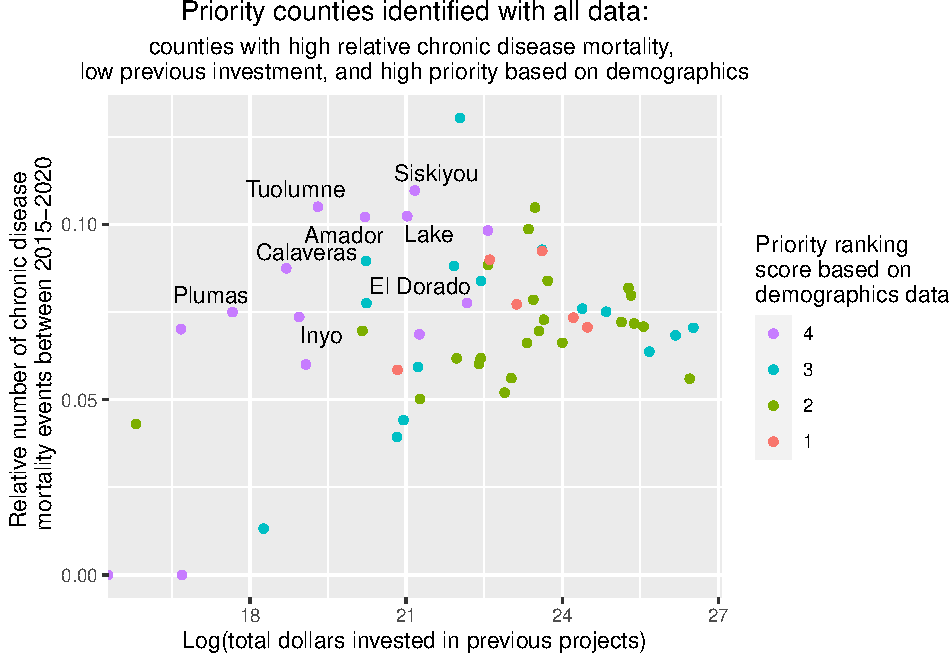
\includegraphics{Milestone-4-R-Project_files/figure-latex/unnamed-chunk-7-1.pdf}

\newpage

\hypertarget{visualization-3}{%
\section{Visualization 3:}\label{visualization-3}}

Table 1: We used a table as a different way to organize the 5 variables
of interest. We categorized each variable and then ranked each as high,
medium, or low priority. We then created a new variable where ``high
priority'' variables were given two points, ``medium priority''
variables given 1 point, and ``low priority'' variables given 0 points
for each county. Then Counties are ranked by number of points. Most of
the Counties highlighted in Plot/Visualization 2 were also the most
highly ranked in the table.

\begin{Shaded}
\begin{Highlighting}[]
\FunctionTok{library}\NormalTok{(kableExtra)}
\end{Highlighting}
\end{Shaded}

\begin{verbatim}
## 
## Attaching package: 'kableExtra'
\end{verbatim}

\begin{verbatim}
## The following object is masked from 'package:dplyr':
## 
##     group_rows
\end{verbatim}

\begin{Shaded}
\begin{Highlighting}[]
\NormalTok{table\_col\_order }\OtherTok{\textless{}{-}} \FunctionTok{c}\NormalTok{(}\StringTok{"county"}\NormalTok{, }\StringTok{"summed\_total\_cost"}\NormalTok{, }\StringTok{"pop12\_sqmi"}\NormalTok{,}
                     \StringTok{"med\_age"}\NormalTok{, }\StringTok{"renter\_ratio"}\NormalTok{,}
                     \StringTok{"relative\_chronic\_dis\_mort"}\NormalTok{, }\StringTok{"med\_age\_CAT"}\NormalTok{,}
                     \StringTok{"summed\_total\_cost\_CAT"}\NormalTok{, }\StringTok{"pop12\_sqmi\_CAT"}\NormalTok{,}
                     \StringTok{"renter\_ratio\_CAT"}\NormalTok{,}\StringTok{"relative\_chronic\_dis\_mort\_CAT"}\NormalTok{)}
\NormalTok{merged\_data\_for\_table }\OtherTok{\textless{}{-}}\NormalTok{ merged\_data[, table\_col\_order]}

\NormalTok{ table}\OtherTok{\textless{}{-}}\NormalTok{merged\_data\_for\_table}\SpecialCharTok{\%\textgreater{}\%}
  \FunctionTok{rowwise}\NormalTok{() }\SpecialCharTok{\%\textgreater{}\%}
  \FunctionTok{mutate}\NormalTok{(}\AttributeTok{number\_highs=} \FunctionTok{sum}\NormalTok{(}\FunctionTok{c\_across}\NormalTok{(}\DecValTok{7}\SpecialCharTok{:}\DecValTok{11}\NormalTok{) }\SpecialCharTok{==} \StringTok{"High priority"}\NormalTok{, }\AttributeTok{na.rm =} \ConstantTok{TRUE}\NormalTok{),}
         \AttributeTok{number\_mediums=} \FunctionTok{sum}\NormalTok{(}\FunctionTok{c\_across}\NormalTok{(}\DecValTok{7}\SpecialCharTok{:}\DecValTok{11}\NormalTok{) }\SpecialCharTok{==} \StringTok{"Medium priority"}\NormalTok{, }\AttributeTok{na.rm =} \ConstantTok{TRUE}\NormalTok{),}
         \AttributeTok{temp\_rank=}\NormalTok{(number\_highs}\SpecialCharTok{*}\DecValTok{2}\NormalTok{)}\SpecialCharTok{+}\NormalTok{number\_mediums}
\NormalTok{         )}\SpecialCharTok{\%\textgreater{}\%}
   \FunctionTok{ungroup}\NormalTok{()}\SpecialCharTok{\%\textgreater{}\%}
   \FunctionTok{arrange}\NormalTok{(}\FunctionTok{desc}\NormalTok{(temp\_rank))}\SpecialCharTok{\%\textgreater{}\%}
   \FunctionTok{select}\NormalTok{(}\SpecialCharTok{{-}}\FunctionTok{c}\NormalTok{(number\_highs, number\_mediums))}\SpecialCharTok{\%\textgreater{}\%}
   \FunctionTok{slice}\NormalTok{(}\DecValTok{1}\SpecialCharTok{:}\DecValTok{15}\NormalTok{)}
\NormalTok{table}
\end{Highlighting}
\end{Shaded}

\begin{verbatim}
## # A tibble: 15 x 12
##    county    summed_total_cost pop12_sqmi med_age renter_ratio relative_chronic~
##    <chr>                 <dbl>      <dbl>   <dbl>        <dbl>             <dbl>
##  1 Amador           598970736.      63.3     48.2        0.253            0.102 
##  2 Calaveras        131848234.      44.6     49.1        0.231            0.0875
##  3 Tuolumne         242129946       24.3     47.1        0.302            0.105 
##  4 Inyo             169160700.       1.82    45.5        0.364            0.0737
##  5 Lake            1347450993.      49.1     45          0.342            0.102 
##  6 Mariposa          17474756       12.6     49.2        0.321            0.0702
##  7 Nevada          6352716267.     103.      47.5        0.280            0.0984
##  8 Plumas            46955168        7.65    49.5        0.305            0.0750
##  9 Siskiyou        1558949981.       7.12    46.8        0.353            0.110 
## 10 Tehama           610226591.      21.5     39.5        0.354            0.0896
## 11 Alpine                   0        1.54    46.4        0.282            0     
## 12 Del Norte        615640530.      28.3     39          0.383            0.0776
## 13 El Dorado       4239088028.     102.      43.5        0.268            0.0776
## 14 Humboldt       17981394511.      38.1     37.3        0.450            0.0929
## 15 Modoc           1703663257        2.33    46          0.314            0.0687
## # ... with 6 more variables: med_age_CAT <fct>, summed_total_cost_CAT <fct>,
## #   pop12_sqmi_CAT <fct>, renter_ratio_CAT <chr>,
## #   relative_chronic_dis_mort_CAT <fct>, temp_rank <dbl>
\end{verbatim}

\begin{Shaded}
\begin{Highlighting}[]
\NormalTok{table }\OtherTok{\textless{}{-}}\NormalTok{ table }\SpecialCharTok{\%\textgreater{}\%} \FunctionTok{select}\NormalTok{(, }\FunctionTok{c}\NormalTok{(}\DecValTok{1}\NormalTok{,}\DecValTok{2}\NormalTok{,}\DecValTok{8}\NormalTok{,}\DecValTok{3}\NormalTok{,}\DecValTok{9}\NormalTok{,}\DecValTok{4}\NormalTok{,}\DecValTok{7}\NormalTok{,}\DecValTok{5}\NormalTok{,}\DecValTok{10}\NormalTok{,}\DecValTok{6}\NormalTok{,}\DecValTok{11}\NormalTok{))}

\FunctionTok{kable}\NormalTok{(table,}
        \AttributeTok{col.names =} \FunctionTok{c}\NormalTok{(}\StringTok{"County"}\NormalTok{,}\StringTok{"Previous spending on projects"}\NormalTok{,}\StringTok{""}\NormalTok{,}
                      \StringTok{"Population density"}\NormalTok{, }\StringTok{""}\NormalTok{,}
                      \StringTok{"Median age of population"}\NormalTok{, }\StringTok{""}\NormalTok{,}
                       \StringTok{"\% population that are renters"}\NormalTok{, }\StringTok{""}\NormalTok{,}
                      \StringTok{"Chronic disease mortality burden"}\NormalTok{, }\StringTok{""}
\NormalTok{                    ),}
       \AttributeTok{caption=}\StringTok{"Top 10 Counties ranked by need for oshpd projects."}\NormalTok{,}
        \AttributeTok{booktabs=}\ConstantTok{TRUE}\NormalTok{,}
        \AttributeTok{align=}\StringTok{\textquotesingle{}lccccc\textquotesingle{}}\NormalTok{)}\SpecialCharTok{\%\textgreater{}\%}
   \FunctionTok{kable\_styling}\NormalTok{(}\AttributeTok{latex\_options=}\StringTok{"scale\_down"}\NormalTok{)}
\end{Highlighting}
\end{Shaded}

\begin{table}

\caption{\label{tab:unnamed-chunk-8}Top 10 Counties ranked by need for oshpd projects.}
\centering
\resizebox{\linewidth}{!}{
\begin{tabular}[t]{lccccclcccc}
\toprule
County & Previous spending on projects &  & Population density &  & Median age of population &  & \% population that are renters &  & Chronic disease mortality burden & \\
\midrule
Amador & 598970736 & High priority & 63.288340 & High priority & 48.2 & High priority & 0.2530030 & Low priority & 0.1021536 & High priority\\
Calaveras & 131848234 & High priority & 44.582939 & High priority & 49.1 & High priority & 0.2311765 & Low priority & 0.0875314 & High priority\\
Tuolumne & 242129946 & High priority & 24.304973 & High priority & 47.1 & High priority & 0.3017241 & Low priority & 0.1051309 & High priority\\
Inyo & 169160700 & High priority & 1.819773 & High priority & 45.5 & High priority & 0.3637719 & Low priority & 0.0736661 & Medium priority\\
Lake & 1347450993 & Medium priority & 49.082334 & High priority & 45.0 & High priority & 0.3418713 & Low priority & 0.1024321 & High priority\\
\addlinespace
Mariposa & 17474756 & High priority & 12.613887 & High priority & 49.2 & High priority & 0.3205512 & Low priority & 0.0701707 & Medium priority\\
Nevada & 6352716267 & Medium priority & 102.564339 & High priority & 47.5 & High priority & 0.2802273 & Low priority & 0.0983582 & High priority\\
Plumas & 46955168 & High priority & 7.653217 & High priority & 49.5 & High priority & 0.3054473 & Low priority & 0.0750500 & Medium priority\\
Siskiyou & 1558949981 & Medium priority & 7.120891 & High priority & 46.8 & High priority & 0.3525250 & Low priority & 0.1097566 & High priority\\
Tehama & 610226591 & High priority & 21.523312 & High priority & 39.5 & Medium priority & 0.3535995 & Low priority & 0.0895902 & High priority\\
\addlinespace
Alpine & 0 & High priority & 1.543841 & High priority & 46.4 & High priority & 0.2816901 & Low priority & 0.0000000 & Low priority\\
Del Norte & 615640530 & High priority & 28.298164 & High priority & 39.0 & Medium priority & 0.3828606 & Low priority & 0.0776015 & Medium priority\\
El Dorado & 4239088028 & Medium priority & 102.156840 & High priority & 43.5 & High priority & 0.2681742 & Low priority & 0.0775971 & Medium priority\\
Humboldt & 17981394511 & Medium priority & 38.062105 & High priority & 37.3 & Medium priority & 0.4499474 & Low priority & 0.0928689 & High priority\\
Modoc & 1703663257 & Medium priority & 2.329272 & High priority & 46.0 & High priority & 0.3144685 & Low priority & 0.0687366 & Medium priority\\
\bottomrule
\end{tabular}}
\end{table}

\end{document}
